\documentclass[tikz,border=4pt]{standalone}
\usepackage[T1]{fontenc}
\usepackage{lmodern}
\renewcommand{\familydefault}{\sfdefault}
\usetikzlibrary{shapes.geometric,positioning,arrows.meta,calc,fit,backgrounds,decorations.pathreplacing}
\tikzset{
  node distance=6mm,
  every node/.style={font=\footnotesize,align=center,execute at begin node={\hyphenpenalty=10000\relax}},
  base/.style={draw=gray!60,fill=gray!12,minimum height=7mm,inner sep=2pt},
  term/.style={base,rounded corners=3.5mm,text width=30mm},
  proc/.style={base,text width=32mm},
  err/.style={base,text width=30mm,fill=gray!22},
  io/.style={base,trapezium,trapezium left angle=72,trapezium right angle=108,trapezium stretches=true,text width=28mm},
  dec/.style={base,diamond,aspect=2.4,text width=27mm,inner sep=0pt},
  % predefined process: a call to another procedure
  sub/.style={proc,inner xsep=3mm,path picture={
    \draw[gray!60] ([xshift=1.5mm]path picture bounding box.north west)--([xshift=1.5mm]path picture bounding box.south west)
                   ([xshift=-1.5mm]path picture bounding box.north east)--([xshift=-1.5mm]path picture bounding box.south east);}},
  go/.style={-{Stealth[length=2mm]},draw=gray!55!black},
  lab/.style={font=\scriptsize,fill=white,inner sep=1pt},
  frame/.style={draw=gray!60,dashed,rounded corners=2mm,inner sep=3mm},
  % memory diagrams
  cell/.style={draw=gray!60,fill=gray!12,minimum height=7mm,inner sep=1pt,font=\scriptsize},
  hot/.style={cell,fill=gray!35},
  note/.style={font=\scriptsize,text=gray!30!black},
}

\begin{document}
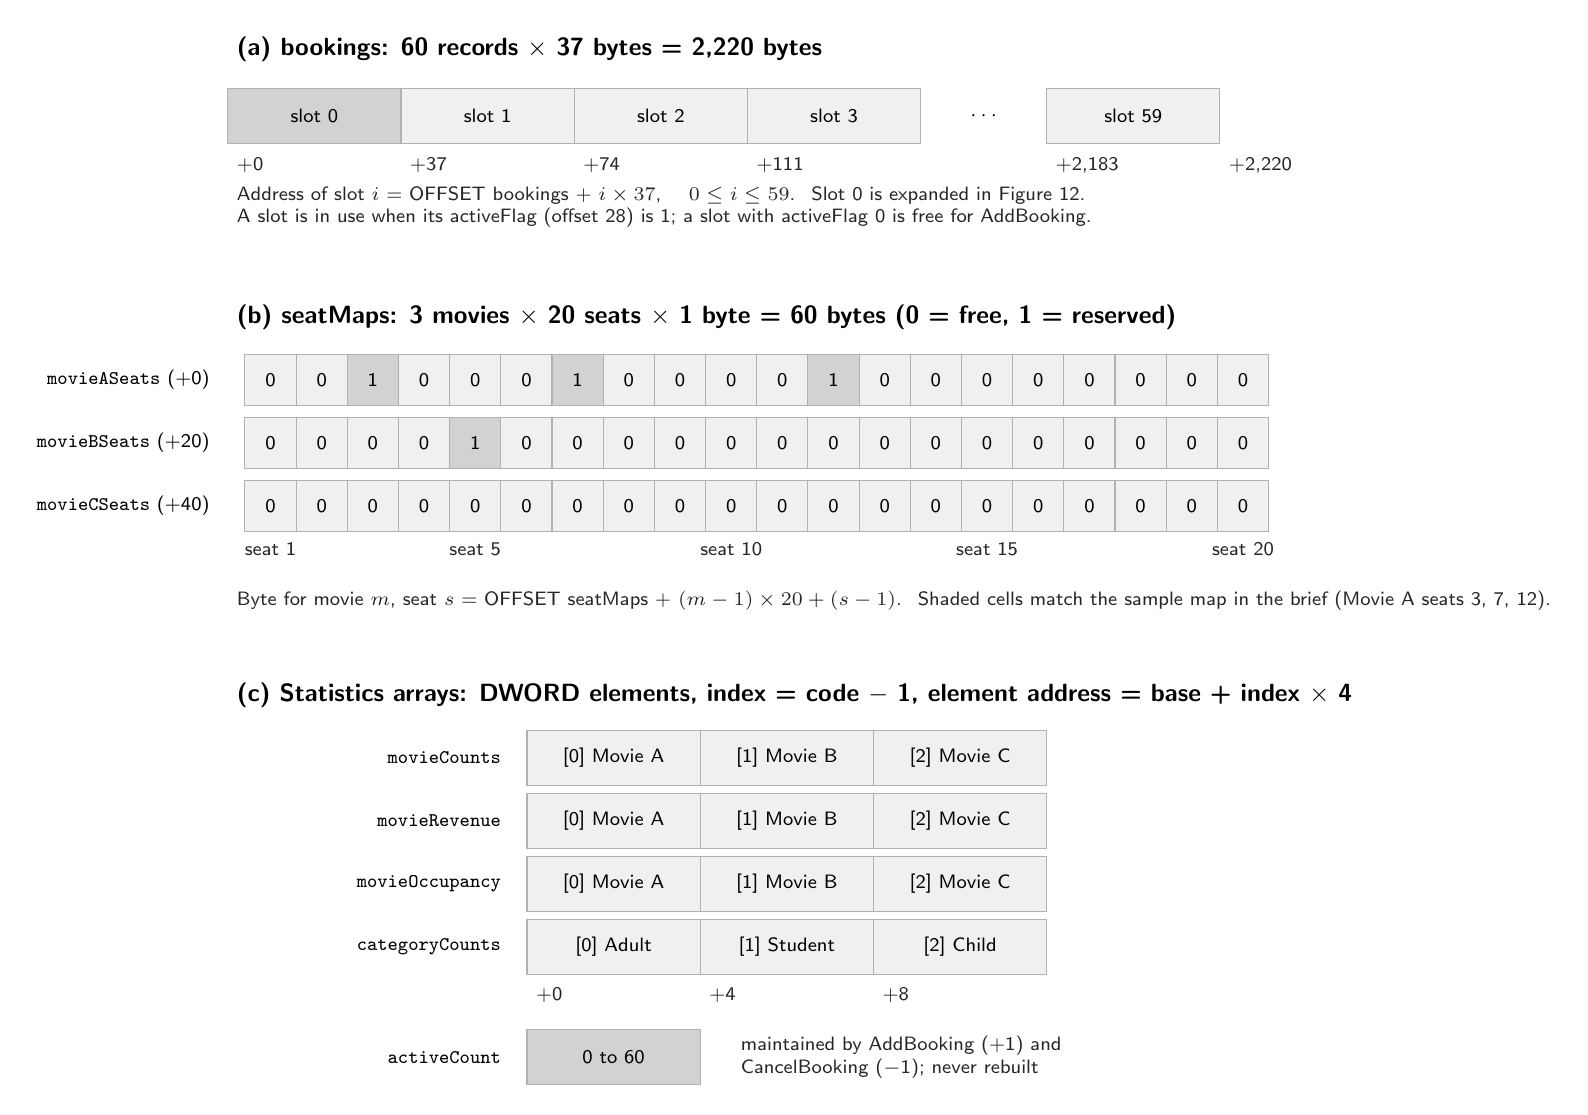
\begin{tikzpicture}[x=1mm,y=1mm]
% ---- (a) booking array
\node[anchor=west,font=\small\bfseries] at (0,12) {(a) bookings: 60 records $\times$ 37 bytes = 2,220 bytes};
\foreach \i/\x/\st/\lab/\off in {0/0/hot/slot 0/+0,1/22/cell/slot 1/+37,2/44/cell/slot 2/+74,3/66/cell/slot 3/+111}{
  \node[\st,minimum width=22mm,anchor=south west] at (\x,0) {\lab};
  \node[note,anchor=north west] at (\x,-0.5) {\off};}
\node[cell,minimum width=16mm,anchor=south west,fill=white,draw=none] at (88,0) {$\cdots$};
\node[cell,minimum width=22mm,anchor=south west] at (104,0) {slot 59};
\node[note,anchor=north west] at (104,-0.5) {+2,183};
\node[note,anchor=north west] at (126,-0.5) {+2,220};
\node[note,anchor=west,align=left] at (0,-8) {Address of slot $i$ = OFFSET bookings + $i \times 37$, \quad $0 \le i \le 59$. \ Slot 0 is expanded in Figure 12.\\A slot is in use when its activeFlag (offset 28) is 1; a slot with activeFlag 0 is free for AddBooking.};
% ---- (b) seat maps
\node[anchor=west,font=\small\bfseries] at (0,-22) {(b) seatMaps: 3 movies $\times$ 20 seats $\times$ 1 byte = 60 bytes (0 = free, 1 = reserved)};
\foreach \m/\lbl/\off [count=\r from 0] in {A/movieASeats/0,B/movieBSeats/20,C/movieCSeats/40}{
  \node[anchor=east,font=\scriptsize] at (-1,-30-\r*8) {\texttt{\lbl} (+\off)};
  \foreach \s in {1,...,20}{
    \pgfmathsetmacro{\v}{(\r==0 && (\s==3 || \s==7 || \s==12)) || (\r==1 && \s==5) ? 1 : 0}
    \ifdim\v pt>0pt \node[hot,minimum width=6.5mm,minimum height=6.5mm] at (\s*6.5-1,-30-\r*8) {1};
    \else \node[cell,minimum width=6.5mm,minimum height=6.5mm] at (\s*6.5-1,-30-\r*8) {0};\fi}}
\foreach \s in {1,5,10,15,20}{\node[note] at (\s*6.5-1,-51.5) {seat \s};}
\node[note,anchor=west,align=left] at (0,-58) {Byte for movie $m$, seat $s$ = OFFSET seatMaps + $(m-1)\times 20 + (s-1)$. \ Shaded cells match the sample map in the brief (Movie A seats 3, 7, 12).};
% ---- (c) statistics arrays
\node[anchor=west,font=\small\bfseries] at (0,-70) {(c) Statistics arrays: DWORD elements, index = code $-$ 1, element address = base + index $\times$ 4};
\foreach \name/\a/\b/\c [count=\r from 0] in {movieCounts/Movie A/Movie B/Movie C,movieRevenue/Movie A/Movie B/Movie C,movieOccupancy/Movie A/Movie B/Movie C,categoryCounts/Adult/Student/Child}{
  \node[anchor=east,font=\scriptsize] at (36,-78-\r*8) {\texttt{\name}};
  \node[cell,minimum width=22mm,anchor=west] at (38,-78-\r*8) {[0] \a};
  \node[cell,minimum width=22mm,anchor=west] at (60,-78-\r*8) {[1] \b};
  \node[cell,minimum width=22mm,anchor=west] at (82,-78-\r*8) {[2] \c};}
\foreach \o/\x in {+0/38,+4/60,+8/82}{\node[note,anchor=north west] at (\x,-106) {\o};}
\node[anchor=east,font=\scriptsize] at (36,-116) {\texttt{activeCount}};
\node[hot,minimum width=22mm,anchor=west] at (38,-116) {0 to 60};
\node[note,anchor=west,align=left] at (64,-116) {maintained by AddBooking (+1) and\\CancelBooking ($-$1); never rebuilt};
\end{tikzpicture}
\end{document}
